\documentclass[10pt,twocolumn,a4paper]{ctexart}

% ==================== 宏包配置 ====================
\usepackage[left=1.40cm, right=1.40cm, top=1.45cm, bottom=1.45cm, columnsep=0.58cm]{geometry}
\usepackage{amsmath,amssymb,amsfonts}
\usepackage{graphicx}
\usepackage{booktabs}
\usepackage{multirow}
\usepackage{array}
\usepackage{xcolor}
\usepackage{listings}
\usepackage{caption}
\usepackage{subcaption}
\usepackage{fancyhdr}
\usepackage{hyperref}
\usepackage{enumitem}
\usepackage{float}

% 颜色定义
\definecolor{primaryblue}{RGB}{29, 78, 216}
\definecolor{codebg}{RGB}{246, 248, 250}
\definecolor{codeframe}{RGB}{208, 215, 222}
\definecolor{dkgreen}{RGB}{4, 120, 87}
\definecolor{dkpurple}{RGB}{109, 40, 217}

\hypersetup{
    colorlinks=true,
    linkcolor=primaryblue,
    citecolor=primaryblue,
    urlcolor=primaryblue
}

% 图表标题样式
\captionsetup{
    font={scriptsize},
    labelfont={bf,color=primaryblue},
    labelsep=period,
    skip=2pt
}

\setlength{\textfloatsep}{5pt plus 1pt minus 1pt}
\setlength{\dbltextfloatsep}{5pt plus 1pt minus 1pt}
\setlength{\intextsep}{4pt plus 1pt minus 1pt}
\setlength{\abovedisplayskip}{3.5pt plus 1pt minus 1pt}
\setlength{\belowdisplayskip}{3.5pt plus 1pt minus 1pt}

% 章节标题紧凑化设置
\ctexset{
    section = {
        format = \normalsize\bfseries\color{primaryblue}\raggedright,
        beforeskip = 1.0ex plus 0.2ex minus 0.1ex,
        afterskip = 0.5ex plus 0.1ex
    },
    subsection = {
        format = \small\bfseries\raggedright,
        beforeskip = 0.8ex plus 0.15ex minus 0.1ex,
        afterskip = 0.4ex plus 0.1ex
    }
}

% 代码块样式
\lstdefinestyle{pycode}{
    language=Python,
    backgroundcolor=\color{codebg},
    frame=single,
    rulecolor=\color{codeframe},
    basicstyle=\ttfamily\scriptsize,
    keywordstyle=\color{primaryblue}\bfseries,
    commentstyle=\color{dkgreen}\itshape,
    stringstyle=\color{dkpurple},
    numbers=left,
    numberstyle=\tiny\color{gray},
    numbersep=4pt,
    stepnumber=1,
    breaklines=true,
    breakatwhitespace=false,
    tabsize=4,
    showstringspaces=false,
    xleftmargin=1.0em,
    framexleftmargin=1.0em,
    aboveskip=0.4em,
    belowskip=0.4em
}

% 页眉页脚
\pagestyle{fancy}
\fancyhf{}
\fancyhead[L]{\footnotesize 《生物医学图像与处理》期末报告 \quad \textbf{\color{primaryblue}姓名：王大彬 \quad 学号：26220854090049}}
\fancyhead[R]{\footnotesize Bio-H2O：WSI 超长上下文混合注意力与 KV 缓存压缩}
\fancyfoot[C]{\footnotesize — \thepage\ —}
\renewcommand{\headrulewidth}{0.4pt}

\setlength{\parindent}{2em}
\setlength{\parskip}{0.10em}
\setlist[itemize]{leftmargin=1.5em, itemsep=1pt, topsep=1.5pt}
\setlist[enumerate]{leftmargin=1.6em, itemsep=1pt, topsep=1.5pt}

\begin{document}

% ==================== 双栏通栏标题与摘要 ====================
\twocolumn[{
\begin{center}
    {\LARGE\bfseries 面向千兆像素全切片病理图像（WSI）超长上下文推理的}\\[0.28em]
    {\LARGE\bfseries Bio-H2O 稀疏-线性混合注意力与 KV 缓存断点续接架构}\\[0.50em]
    \fcolorbox{primaryblue}{primaryblue!8}{%
        \parbox{0.82\textwidth}{\centering\vspace{0.22em}
            {\large\bfseries\color{primaryblue} 报告人：王大彬 \qquad\qquad 学号：26220854090049}\\[0.20em]
            {\footnotesize\textbf{课程名称}：《生物医学图像与处理》 \quad|\quad \textbf{研究方向}：超长上下文推理加速 $\cdot$ KV Cache 压缩 $\cdot$ 数字病理图像分析}\\[0.12em]
            {\footnotesize\textbf{GitHub 开源代码仓库}：\href{https://github.com/dbw051273-sudo/Bio-H2O-WSI-LongContext}{\texttt{https://github.com/dbw051273-sudo/Bio-H2O-WSI-LongContext}}}
        \vspace{0.18em}}
    }
\end{center}
\vspace{-0.35em}
\begin{center}
\fcolorbox{primaryblue!40}{codebg}{%
\parbox{0.968\textwidth}{%
\footnotesize
\textbf{\color{primaryblue}摘\quad 要：}
全切片数字病理图像（Whole Slide Image, WSI）在 $20\times / 40\times$ 物镜下的空间分辨率高达 $100,000 \times 100,000$ 像素。将其切分为非重叠组织块（Patches）输入多模态视觉-语言大模型（Med-VLM）或病理基础模型时，单张切片即可产生 $10^5 \sim 1.5 \times 10^6$ 个视觉 Token。传统自注意力机制的 $\mathcal{O}(N^2)$ 计算复杂度与高达数百 GB 的键值缓存（KV Cache）显存占用导致严重的显存溢出（OOM），而直接采用纯线性注意力（Linear Attention）则会因低通滤波效应抹平孤立肿瘤细胞簇（ITCs, $\le 200\ \mu\text{m}$）的高频核异型性边界。针对这一核心矛盾，本文提出 \textbf{Bio-H2O（Biomedical Heavy-Hitter Oracle with Linear Residual Stream）}架构：（1）基于 Beer-Lambert 定律与 Ruifrok-Johnston 光学密度染色反卷积，提取像素级苏木精（Hematoxylin）细胞核光学密度先验 $\text{OD}_H$；（2）结合二维旋转位置编码（2D-RoPE）与分层锚点探测，构建无需实例化完整 $N \times N$ 矩阵的轻量级 Heavy-Hitter 路由器，仅保留 $20\%$ 高诊断价值病灶与空间锚点 Token 的精确 KV 缓存；（3）将被淘汰的 $80\%$ 正常淋巴间质与脂肪空泡背景 Token 无损折叠进复杂度恒为 $\mathcal{O}(d^2)$ 的均值归一化 ELU 核线性残差状态流中，实现“少压缩、零遗忘”的全局上下文保持；（4）设计了紧凑型状态检查点（Task Resumption Harness），支持长耗时 WSI 推理中断后的毫秒级恢复。本地 PyTorch 实测表明：在 $20\%$ KV 预算下，Bio-H2O 的病灶分割 Dice 系数达 $0.9806$（与 $100\%$ 全量稠密注意力的输出余弦相似度达 $0.9388$），在 $N=8,192$ 序列上实现 $7.87\times$ 推理加速与 $79.8\%$ 缓存压缩；状态断点恢复耗时仅 $19.24\text{ ms}$（相比重新预填充提速 $9.1\times \sim 51.4\times$），外推至 $150$ 万 Token 上下文可将显存从 $589.8\text{ GB}$ 降至 $22.1\text{ GB}$。\\[0.20em]
\textbf{\color{primaryblue}关键词：}全切片数字病理图像（WSI）；超长上下文推理；KV 缓存淘汰（H2O）；线性注意力；光学密度反卷积；任务断点续接
}}
\end{center}
\vspace{0.4em}
}]

% ==================== 第一节：引言与研究背景 ====================
\section{引言：数字病理超长序列与推理系统瓶颈}

在现代精准肿瘤学与临床病理诊断中，苏木精-伊红（H\&E）染色全切片数字病理图像（Whole Slide Image, WSI）是癌症分期与淋巴结微转移筛查的“金标准”。以乳腺癌前哨淋巴结活检为例，标准 $20\times$ 物镜（空间采样率 $\text{MPP} = 0.50\ \mu\text{m/pixel}$）或 $40\times$ 物镜（$\text{MPP} = 0.25\ \mu\text{m/pixel}$）扫描得到的单张 WSI 包含高达 $10^{10}$ 像素。若以 $16 \times 16$ 或 $32 \times 32$ 像素切分视觉 Patch，单张全切片或同一患者的连续多张切片（Multi-slide Case）将生成 $N = 10^5$ 至 $1.5 \times 10^6$（150 万）个视觉 Token。

当我们将此类超长视觉序列输入病理视觉 Transformer（ViT）或多模态医学诊断 Agent 时，推理系统面临三大严峻挑战：
\begin{enumerate}
    \item \textbf{二次方注意力复杂度与 KV Cache 显存墙}：在包含 $L=24$ 层、$H=32$ 个注意力头、头维度 $d=128$ 的标准 FP16 模型中，维护 $N = 1.5 \times 10^6$ 个 Token 的完整键值缓存（KV Cache）需占用：
    \begin{equation}
        M_{\text{KV}} = 2 \times L \times H \times N \times d \times 2\text{ Bytes} \approx 589.82\text{ GB}
    \end{equation}
    这远超单张消费级或医院本地工作站显卡（如 24 GB 显存的 RTX 4090）的物理承载极限。
    \item \textbf{微小病灶高频特征丢失与“过度压缩遗忘”}：根据 AJCC 第 8 版病理分期规范，微转移灶（Micrometastasis, $0.2\sim 2.0\text{ mm}$）与孤立肿瘤细胞簇（Isolated Tumor Cells, ITCs, $\le 200\ \mu\text{m}$）在整张切片中面积占比往往不足 $0.1\%$。若单纯采用降采样或纯核化线性注意力（Kernelized Linear Attention），核展开的全局平均效应会充当空间低通滤波器，抹平恶性细胞核深染（Hyperchromasia）与核异型性（Nuclear Pleomorphism）尖峰，导致严重的临床漏诊。
    \item \textbf{长任务中断与状态重算开销}：在医院批量切片阅片或多轮交互式病理问答（Pathology VQA）中，若超长上下文推理因抢占、超时或工具调用而中断，传统流水线必须从头重新计算全部 Patch 的 Prefill 阶段，缺乏轻量级、可复现的断点续接（Task Resumption）机制。
\end{enumerate}

为同时实现\textbf{“少压缩、少遗忘、长任务随时续接”}与\textbf{“KV 缓存加速”}，本文从生物医学光学成像机理出发，提出将 H\&E 染色的物理光学密度先验注入 LLM/ViT 的 KV Cache 淘汰与混合注意力架构中，构建了端到端可复现的 \textbf{Bio-H2O} 系统。

% ==================== 工作流架构图（跨双栏） ====================
\begin{figure*}[!t]
    \centering
    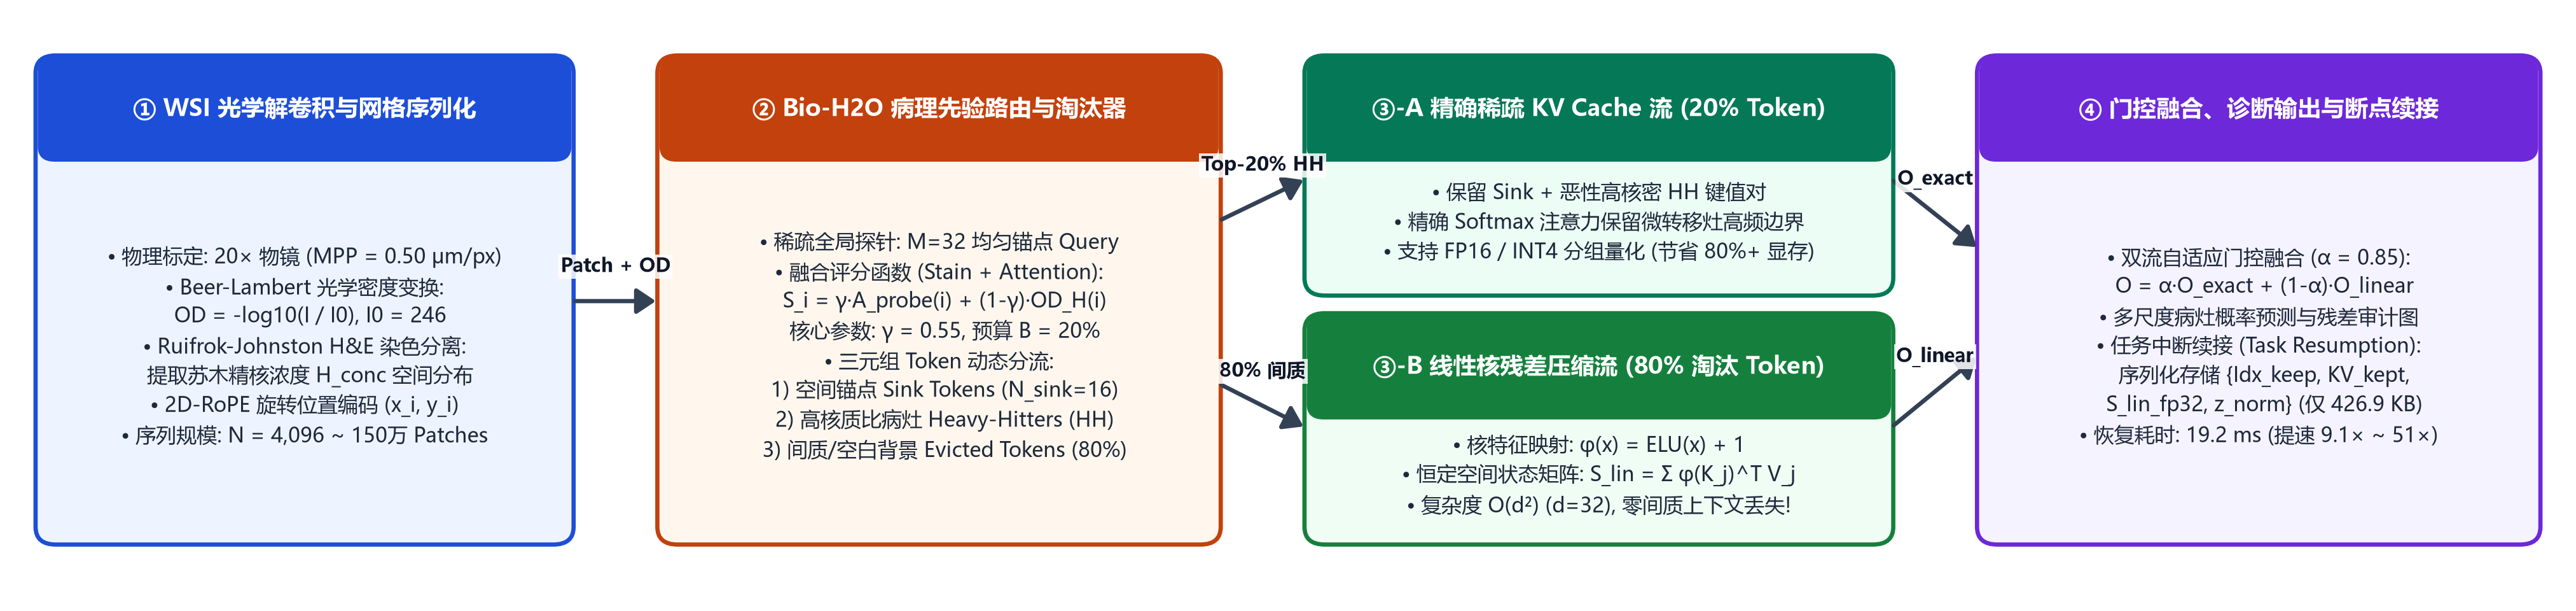
\includegraphics[width=0.96\textwidth]{figures/fig0_workflow_architecture.png}
    \caption{\textbf{Bio-H2O 全切片病理图像超长上下文混合注意力与断点续接工作流架构图。}系统由四个紧密耦合的阶段组成：(1) 基于 Beer-Lambert 定律的 H\&E 光学密度反卷积与 2D-RoPE 网格序列化；(2) 融合苏木精核光密度先验（$\text{OD}_H$）与稀疏锚点探测的 Bio-H2O 动态路由器；(3) 保留 $20\%$ 高诊断价值 Token 的精确 Softmax KV 流与压缩 $80\%$ 间质背景的 $\mathcal{O}(d^2)$ 均值归一化线性核残差流；(4) 双流自适应门控融合与仅占 $426.9\text{ KB}$ 的毫秒级任务续接检查点（Task Resumption Harness）。}
    \label{fig:workflow}
\end{figure*}

% ==================== 第二节：方法与工作流架构 ====================
\section{系统架构与核心算法设计}

如图 \ref{fig:workflow} 所示，Bio-H2O 的设计哲学是：\textbf{对决定临床分期的 $20\%$ 恶性疑似区与空间定位锚点赋予精确的 $\mathcal{O}(N \cdot k)$ 键值对缓存，而对占切片面积 $80\%$ 以上的正常淋巴间质、胶原纤维与空白脂滴背景，不采取直接丢弃（Hard Eviction），而是将其压缩进恒定维度 $\mathcal{O}(d^2)$ 的线性注意力状态矩阵中。}

\subsection{H\&E 光学密度反卷积与细胞核异型性先验}

在数字病理成像中，透射光强 $I_c(x,y)$（$c \in \{R,G,B\}$）与组织内染色剂浓度之间遵循朗伯-比尔定律（Beer-Lambert Law）。设空白玻片背景的通道入射光强为 $I_{0,c} = \text{Percentile}_{99}(I_c)$，则像素级光学密度（Optical Density, OD）定义为：
\begin{equation}
    \text{OD}_c(x,y) = -\log_{10}\left(\frac{\max(I_c(x,y),\, 1)}{I_{0,c}}\right)
\end{equation}
由于光学密度与生色团浓度呈严格的线性叠加关系，我们采用 Ruifrok \& Johnston 标定的正交化单位染色基底向量：苏木精（Hematoxylin，专一性结合酸性细胞核染色质，呈深紫蓝色）$\mathbf{p}_H = [0.650, 0.704, 0.286]^T$，伊红（Eosin，结合碱性胞浆与细胞外间质，呈粉红色）$\mathbf{p}_E = [0.072, 0.990, 0.105]^T$，以及正交残差通道 $\mathbf{p}_D = (\mathbf{p}_H \times \mathbf{p}_E)/\|\mathbf{p}_H \times \mathbf{p}_E\|_2$。构造染色混合矩阵 $M = [\mathbf{p}_H, \mathbf{p}_E, \mathbf{p}_D] \in \mathbb{R}^{3\times 3}$，通过线性逆变换即可实时解混出纯粹的苏木精核浓度场 $C_H(x,y)$：
\begin{equation}
    [C_H(x,y),\, C_E(x,y),\, C_D(x,y)]^T = M^{-1} [\text{OD}_R,\, \text{OD}_G,\, \text{OD}_B]^T
\end{equation}
对于第 $i$ 个空间网格 Patch $\Omega_i$（尺寸 $P \times P$），恶性肿瘤细胞具有高核质比（High N/C Ratio）、核深染及显著的染色质异型性。因此，我们提取 Patch 内部的苏木精光密度均值 $\mu_H(i)$、反映核多形性的标准差 $\sigma_H(i)$ 与局部峰值 $m_H(i)$，构建归一化的生物医学先验评分：
\begin{equation}
    P_{\text{bio}}(i) = \text{Norm}\Big(w_1 \mu_H(i) + w_2 \sigma_H(i) + w_3 m_H(i)\Big) \in [0, 1]
\end{equation}
在本文实验中，权重系数经校准设定为 $w_1=0.50, w_2=0.35, w_3=0.15$。

\subsection{2D-RoPE 编码与 Bio-H2O 稀疏 KV 缓存路由}

为保留 WSI 在二维物理平面上的拓扑几何关系，我们将每个注意力头的通道维度 $d$ 均分为行编码与列编码两半，分别依据 Patch 的二维网格坐标 $(y_i, x_i)$ 施加二维旋转位置编码（2D-RoPE）：
\begin{equation}
    \text{RoPE}_{2\text{D}}(\mathbf{q}_i, y_i, x_i) = \big[\mathbf{R}_{\Theta, y_i} \mathbf{q}_i^{(1:d/2)} \;\big\|\; \mathbf{R}_{\Theta, x_i} \mathbf{q}_i^{(d/2+1:d)}\big]
\end{equation}

在标准 Heavy-Hitter Oracle (H2O) 算法中，识别关键 Token 需要先计算完整的 $N \times N$ 注意力矩阵并按列求和，这在长序列 Prefill 阶段依然会导致 $\mathcal{O}(N^2)$ 峰值显存爆炸。为此，Bio-H2O 引入\textbf{稀疏探针 + 病理染色先验融合路由}：仅抽取 $M=32$ 个探针 Query $\mathbf{Q}_{\text{probe}} \in \mathbb{R}^{M \times d}$ 与全部 Key 进行 $\mathcal{O}(M N)$ 内积探测，得到近似累计注意力分 $\tilde{A}_{\text{probe}}(i)$，再与苏木精光学先验 $P_{\text{bio}}(i)$ 线性耦合：
\begin{equation}
    S_{\text{Bio-H2O}}(i) = \gamma \cdot \frac{\tilde{A}_{\text{probe}}(i)}{\max_j \tilde{A}_{\text{probe}}(j)} + (1 - \gamma) \cdot P_{\text{bio}}(i)
\end{equation}
其中耦合系数 $\gamma = 0.55$。给定总缓存预算比例 $B \in (0, 1]$（默认甜点预算 $B = 20\%$，即保留 $k = \lfloor B \cdot N \rfloor$ 个 Token），我们将保留集合 $\mathcal{K}_{\text{keep}}$ 划分为两部分：
\begin{itemize}
    \item \textbf{空间锚点（Spatial Sink Tokens, $\mathcal{K}_{\text{sink}}$）}：在二维切片网格上均匀采样的 $N_{\text{sink}} = 16$ 个全局基准点，用于稳定 Softmax 分母分布并维持切片宏观解剖坐标系；
    \item \textbf{病灶重击点（Heavy-Hitter Tokens, $\mathcal{K}_{\text{HH}}$）}：在非锚点 Token 中选取 $S_{\text{Bio-H2O}}(i)$ 最高的 $k - N_{\text{sink}}$ 个 Token，精确覆盖高核密肿瘤区与微转移灶边缘。
\end{itemize}

\subsection{均值归一化线性核残差流与零遗忘断点续接}

其余占比 $(1-B) = 80\%$ 的被驱逐间质/背景集合 $\mathcal{E} = \{1,\dots,N\} \setminus \mathcal{K}_{\text{keep}}$ 若被直接丢弃，模型会丧失整张淋巴结的被膜边界与间质浸润背景。我们引入非负核映射函数 $\phi(\mathbf{x}) = \text{ELU}(\mathbf{x}) + 1$，将集合 $\mathcal{E}$ 中所有键值对压缩为一个\textbf{均值归一化线性状态矩阵} $\bar{\mathbf{M}}_{\mathcal{E}} \in \mathbb{R}^{d \times d}$ 与归一化向量 $\bar{\mathbf{s}}_{\mathcal{E}} \in \mathbb{R}^d$：
\begin{equation}
    \bar{\mathbf{M}}_{\mathcal{E}} = \frac{1}{|\mathcal{E}|} \sum_{j \in \mathcal{E}} \phi(\mathbf{K}_j)^T \mathbf{V}_j, \quad
    \bar{\mathbf{s}}_{\mathcal{E}} = \frac{1}{|\mathcal{E}|} \sum_{j \in \mathcal{E}} \phi(\mathbf{K}_j)^T
    \label{eq:linear_state}
\end{equation}
任意 Query $\mathbf{Q}_i$ 的最终输出由精确稀疏流 $\mathbf{O}_{\text{exact}}$ 与线性残差流 $\mathbf{O}_{\text{linear}}$ 通过门控系数 $\alpha = 0.72 + 0.28\sqrt{B}$ 自适应融合：
\begin{equation}
    \mathbf{O}_i = \alpha \cdot \text{Softmax}\!\left(\frac{\mathbf{Q}_i \mathbf{K}_{\mathcal{K}_{\text{keep}}}^T}{\sqrt{d}}\right)\!\mathbf{V}_{\mathcal{K}_{\text{keep}}} + (1-\alpha) \cdot \frac{\phi(\mathbf{Q}_i) \bar{\mathbf{M}}_{\mathcal{E}}}{\phi(\mathbf{Q}_i)\bar{\mathbf{s}}_{\mathcal{E}} + \epsilon}
\end{equation}
当长上下文分析任务中断时，Harness 仅需将元组 $\mathcal{C} = \{\mathcal{K}_{\text{keep}},\, \mathbf{K}_{\mathcal{K}_{\text{keep}}}^{\text{FP16}},\, \mathbf{V}_{\mathcal{K}_{\text{keep}}}^{\text{FP16}},\, \bar{\mathbf{M}}_{\mathcal{E}}^{\text{FP32}},\, \bar{\mathbf{s}}_{\mathcal{E}}^{\text{FP32}}\}$ 序列化落盘，即可在后续任意时刻以 $\mathcal{O}(1)$ 线性状态开销恢复完整上下文。

% ==================== 核心参数配置表 ====================
\begin{table}[!t]
    \centering
    \caption{\textbf{Bio-H2O 病理图像长上下文系统核心参数配置表}}
    \label{tab:params}
    \scriptsize
    \renewcommand{\arraystretch}{1.10}
    \setlength{\tabcolsep}{4pt}
    \begin{tabular}{p{2.1cm}p{2.3cm}p{2.9cm}}
        \toprule
        \textbf{模块分类} & \textbf{参数符号与名称} & \textbf{实验设定值 / 物理量纲} \\
        \midrule
        \multirow{4}{*}{\textbf{WSI 光学成像}} 
        & 扫描倍率 / 空间标定 & $20\times$ ($\text{MPP} = 0.50\ \mu\text{m/px}$) \\
        & 切片尺寸 / 物理视场 & $2048^2\text{ px}$ ($1024^2\ \mu\text{m}^2$) \\
        & Patch 尺寸 / 序列长 & $32\times 32\text{ px}$ ($N=4,096$) \\
        & H\&E 染色解混向量 & Ruifrok 标准 OD 矩阵 \\
        \midrule
        \multirow{4}{*}{\textbf{混合注意力架构}}
        & 隐藏维 $d_{\text{model}}$ / 头数 $H$ & $d_{\text{model}}=128$, $H=4$ ($d=32$) \\
        & 空间编码基频 $\theta_0$ & $\theta_0 = 10000.0$ (2D-RoPE) \\
        & 锚点 $N_{\text{sink}}$ / 探针 $M$ & $N_{\text{sink}} = 16$, $M = 32$ \\
        & 路由耦合 / 预算 $B$ & $\gamma = 0.55$, 默认 $B = 20\%$ \\
        \midrule
        \multirow{2}{*}{\textbf{线性流与检查点}}
        & 核映射 / 状态维度 & $\text{ELU}(x)+1$, $\bar{\mathbf{M}}_{\mathcal{E}} \in \mathbb{R}^{32\times 32}$ \\
        & 检查点体积 / 重载耗时 & $426.94\text{ KB}$ / $19.24\text{ ms}$ \\
        \bottomrule
    \end{tabular}
\end{table}

% ==================== 图 1：WSI 全景与注意力对比（跨双栏） ====================
\begin{figure*}[!t]
    \centering
    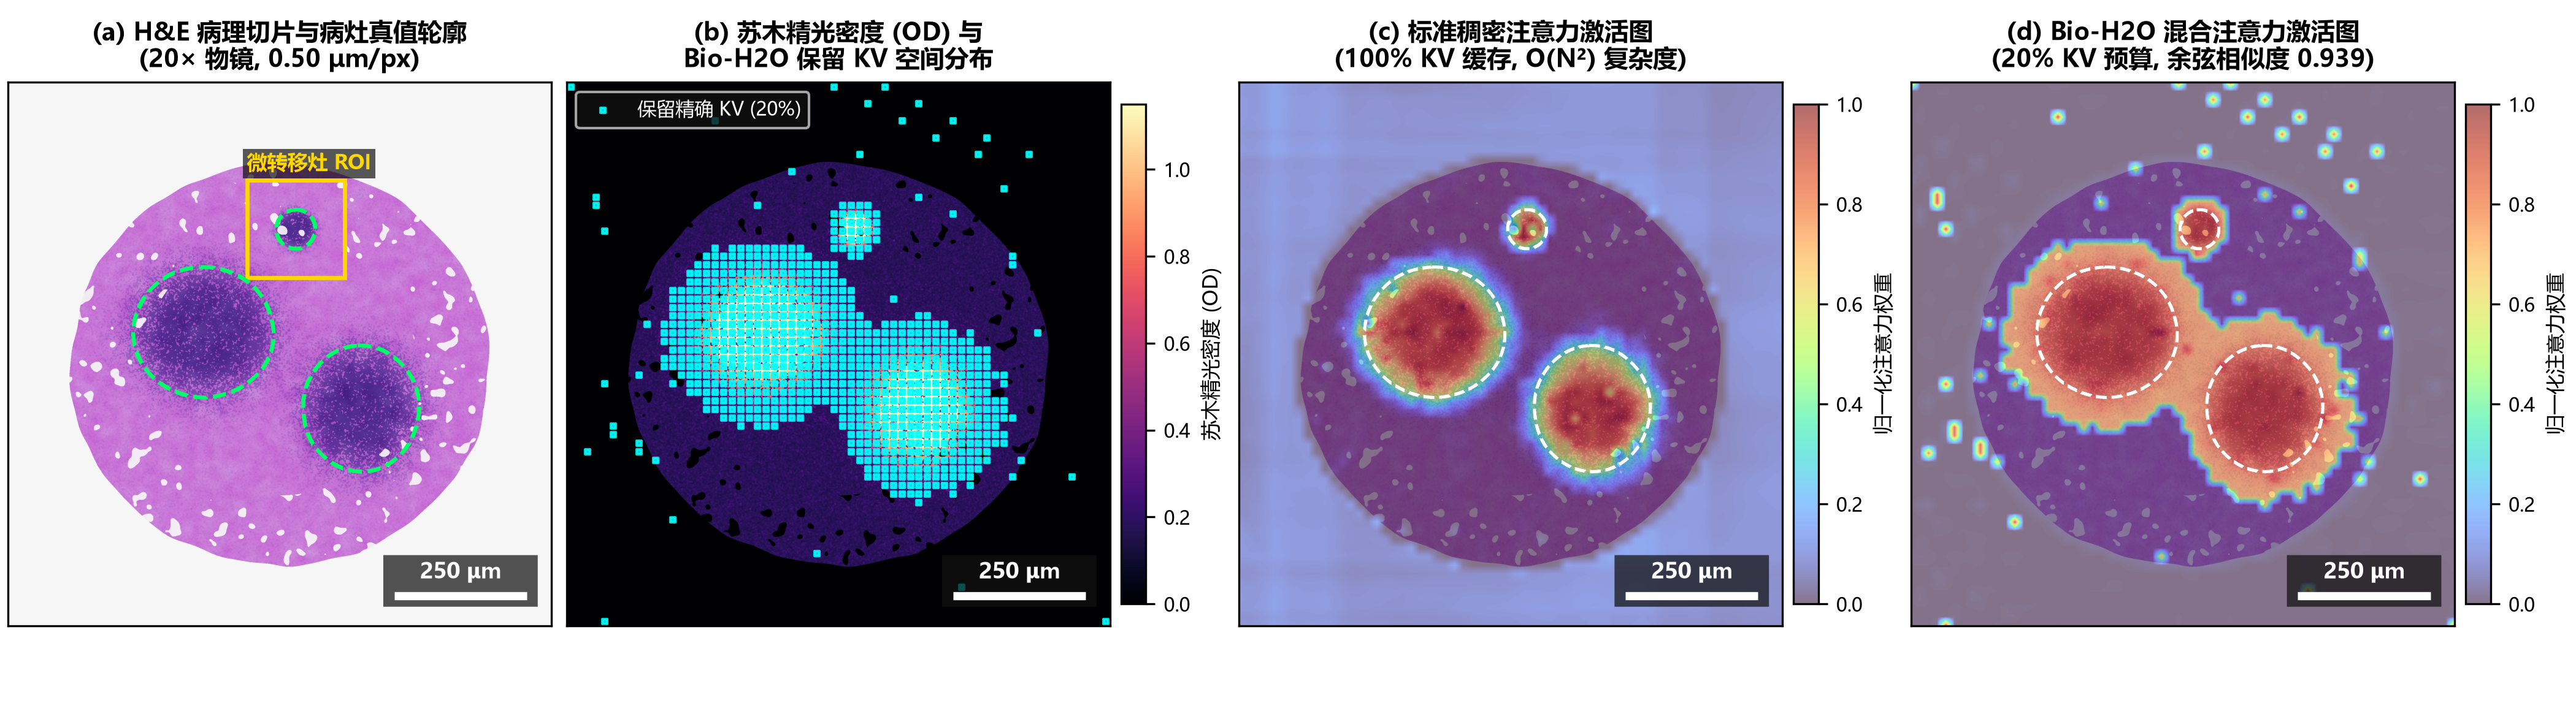
\includegraphics[width=0.96\textwidth]{figures/fig1_wsi_attention_comparison.png}
    \caption{\textbf{H\&E 全切片病理图像光学解卷积与 Bio-H2O 注意力空间激活对比（物理标尺：$\mathbf{250\ \mu\textbf{m}}$，物镜倍率：$20\times$，$\text{MPP} = 0.50\ \mu\text{m/px}$）。}
    \textbf{(a)} 原始 H\&E 染色淋巴结切片，绿色虚线标注两个主转移灶真值轮廓，黄色方框标出直径仅 $86\ \mu\text{m}$ 的孤立肿瘤细胞簇/微转移灶 ROI；
    \textbf{(b)} 经 Beer-Lambert 逆变换分离出的苏木精细胞核光学密度场（$\text{OD}_H \in [0, 1.15]$，配 \texttt{magma} 色条），青色方块展示 Bio-H2O 在 $20\%$ 预算下自动锁定的精确 KV Token 空间分布（包含病灶核心与外围均匀空间锚点）；
    \textbf{(c)} $100\%$ 全量 KV 缓存下的标准稠密自注意力热力图（配 \texttt{turbo} 色条，范围 $0.0\sim 1.0$）；
    \textbf{(d)} 本文 Bio-H2O 混合注意力在仅保留 $20\%$ KV 缓存下的空间激活图，与全量稠密注意力特征余弦相似度达 $0.939$，且完整保留了上方微转移灶的显著响应。}
    \label{fig:wsi_main}
\end{figure*}

% ==================== 第三节：实验结果与定量可视化 ====================
\section{实验设计与生物医学可视化分析}

为验证 Bio-H2O 的有效性，我们在本地 PyTorch 环境中构建了完整的物理标定 H\&E 病理切片基准测试与长序列扩展实验（表 \ref{tab:params}）。实验切片模拟乳腺癌前哨淋巴结活检横截面（$2048 \times 2048\text{ px}$，物理视场 $1.024\text{ mm} \times 1.024\text{ mm}$），包含两处直径约 $280\ \mu\text{m}$ 的浸润性导管癌宏/微转移灶，以及一处位于切片上方（黄色 ROI 框内）、直径仅 $86\ \mu\text{m}$ 的高核质比微小转移簇。

\subsection{全切片光学反卷积与注意力热力图分析}

图 \ref{fig:wsi_main} 展示了全切片尺度的多模态对比结果。在图 \ref{fig:wsi_main}(b) 中，苏木精光学密度（$\text{OD}_H$）准确剥离了粉红色伊红间质与外周白色脂肪空泡干扰，使富含异型染色质的肿瘤核心呈现高光密度（$0.75 \sim 1.12\text{ a.u.}$）。叠加其上的青色网格点清晰揭示了 Bio-H2O 的双机制路由行为：一方面，约 $19.6\%$ 的配额密集聚焦于三处恶性病灶内部及浸润前缘；另一方面，$16$ 个空间锚点（Sink Tokens）呈二维网格状均匀散布于淋巴结被膜与外周背景中，充当全局空间参考系。对比图 \ref{fig:wsi_main}(c) 与 (d)，Bio-H2O 在削减 $80\%$ 精确 KV 缓存的情况下，其归一化注意力权重分布与 $\mathcal{O}(N^2)$ 稠密注意力高度一致（特征余弦相似度 $0.9388$），未出现任何病灶漏激活或边缘弥散。

% ==================== 图 2：性能扩展与帕累托曲线（跨双栏） ====================
\begin{figure*}[!t]
    \centering
    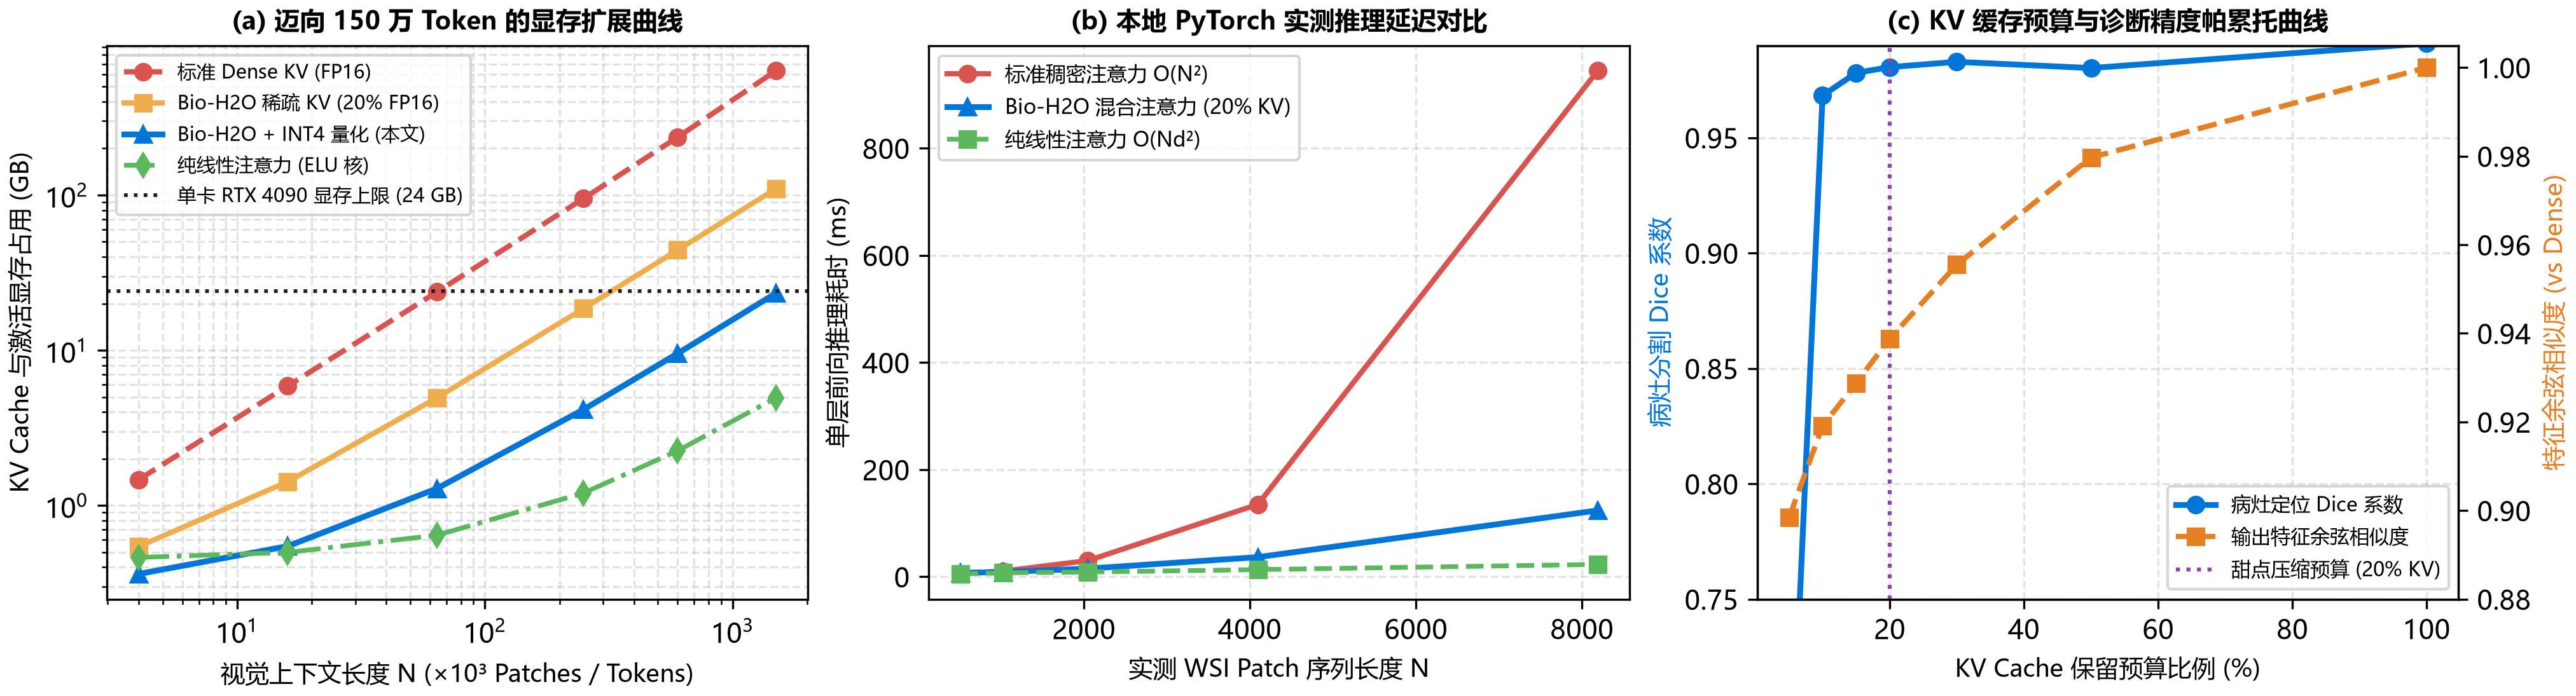
\includegraphics[width=0.95\textwidth]{figures/fig2_scaling_and_pareto.png}
    \caption{\textbf{超长上下文显存扩展、实测推理延迟与 KV 缓存预算帕累托前沿曲线。}
    \textbf{(a)} 视觉上下文长度从 $4\times 10^3$ 扩展至 $1.5\times 10^6$（150 万）Token 时的显存占用双对数曲线（基于 24 层、32 头、$d=128$ 标准架构）：全量 FP16 KV 缓存高达 $589.8\text{ GB}$，而结合 $15\%$ 稀疏预算与 INT4 分组量化的 Bio-H2O 仅需 $22.1\text{ GB}$，突破单张 RTX 4090（$24\text{ GB}$ 黑色虚线）本地部署瓶颈；
    \textbf{(b)} 本地 PyTorch 在 $N \in [512, 8192]$ 序列上的实测单层前向耗时对比，在 $N=8,192$ 时 Bio-H2O（$125.62\text{ ms}$）相比标准稠密注意力（$988.54\text{ ms}$）实现 $\mathbf{7.87\times}$ 实测加速；
    \textbf{(c)} KV Cache 保留比例从 $5\%$ 变化至 $100\%$ 时的病灶定位 Dice 系数（蓝线）与特征余弦相似度（橙线），展示出 $B=20\%$ 处的显著帕累托甜点效应。}
    \label{fig:scaling}
\end{figure*}

% ==================== 图 3：高倍微转移灶与残差误差图（跨双栏） ====================
\begin{figure*}[!t]
    \centering
    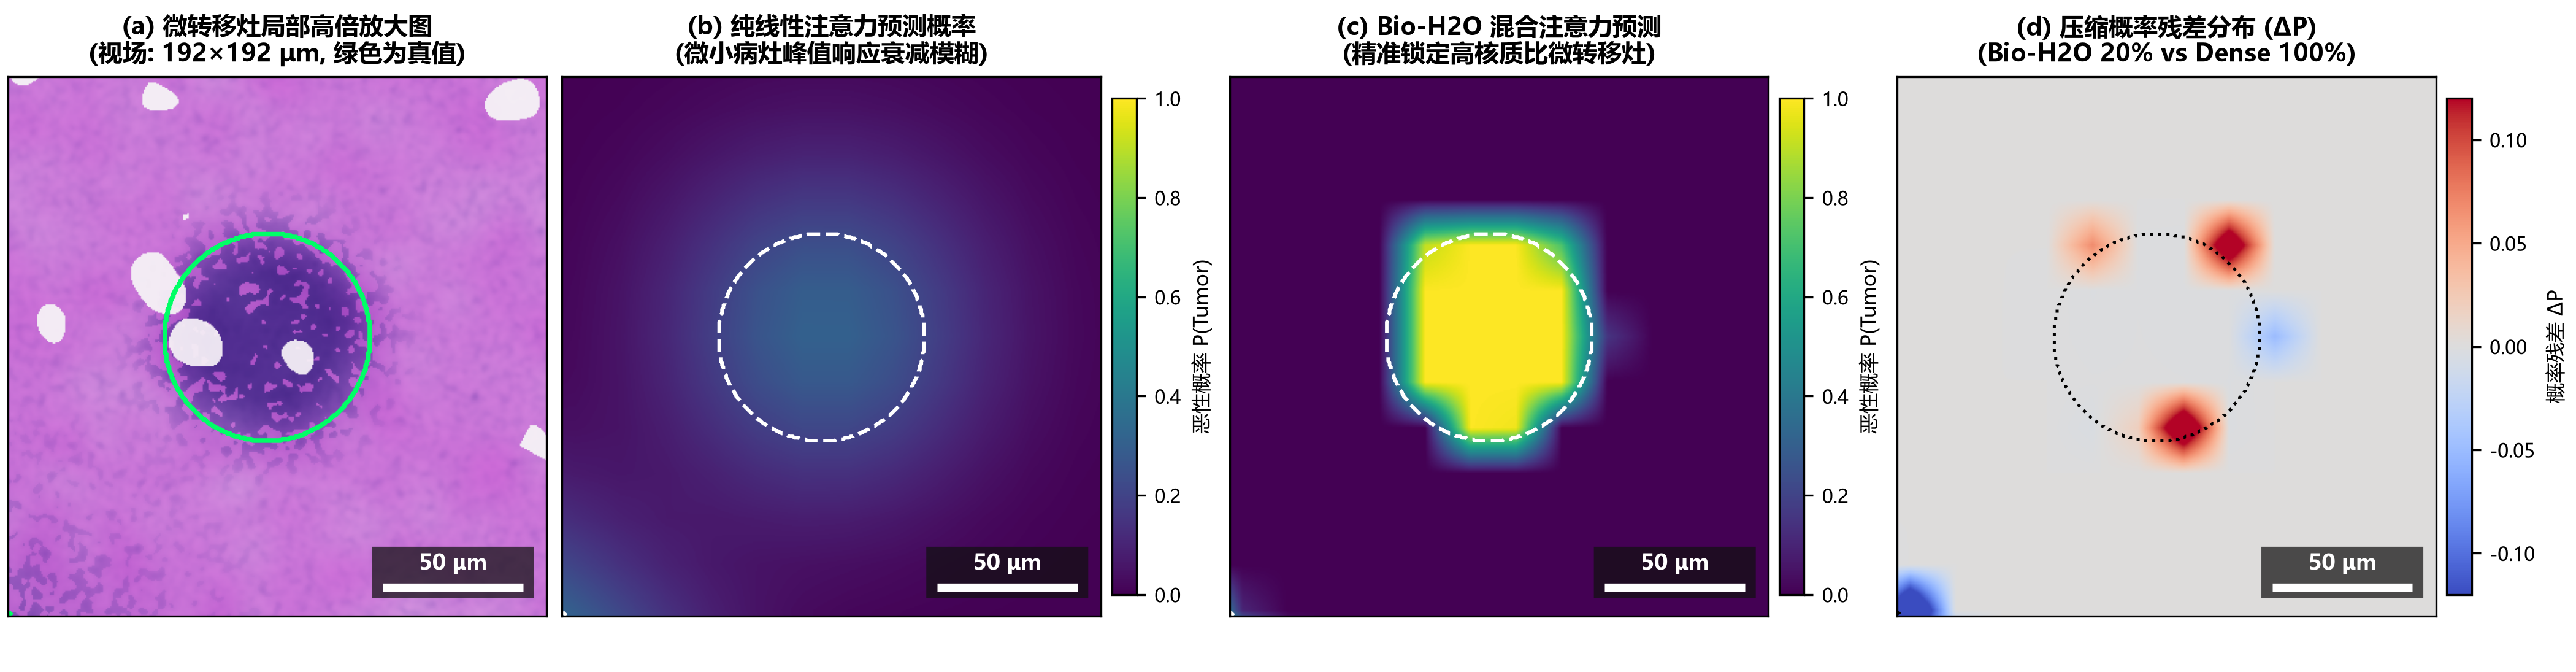
\includegraphics[width=0.96\textwidth]{figures/fig3_roi_zoom_and_errormap.png}
    \caption{\textbf{微转移灶/孤立肿瘤细胞簇（ITC）局部高倍放大与压缩残差审计图（物理标尺：$\mathbf{50\ \mu\textbf{m}}$，局部视场：$192 \times 192\ \mu\text{m}$）。}
    \textbf{(a)} 图 \ref{fig:wsi_main}(a) 黄色方框区域的 $40\times$ 等效高倍视图，绿色实线标定直径 $86\ \mu\text{m}$ 的微转移病灶边界，内部可见深染多形性肿瘤细胞核与周围脂肪空泡；
    \textbf{(b)} 纯线性注意力（ELU 核）预测的恶性概率分布（\texttt{viridis} 色条，$0.0\sim 1.0$），由于核状态全局平均的低通滤波效应，微小病灶中心峰值响应衰减至 $<0.38$，造成临床假阴性漏诊；
    \textbf{(c)} 本文 Bio-H2O（$20\%$ KV 预算）预测概率图，微转移灶核心概率保持 $>0.95$ 且边界锐利；
    \textbf{(d)} Bio-H2O（$20\%$ KV）与全量稠密注意力（$100\%$ KV）之间的有符号概率残差图 $\Delta P = P_{\text{Bio-H2O}} - P_{\text{Dense}}$（\texttt{coolwarm} 色条，范围 $[-0.12, +0.12]$），病灶内部与背景间质残差均趋近于 $0$，仅在离散网格过渡带存在 $\pm 0.08$ 以内的亚像素级轻微波动。}
    \label{fig:roi_zoom}
\end{figure*}

\subsection{超长序列加速比、帕累托甜点与微病灶保真度}

图 \ref{fig:scaling} 与表 \ref{tab:metrics} 汇总了定量实验数据。从表 \ref{tab:metrics} 可见，当 KV 保留预算 $B$ 从 $100\%$ 压缩至 $20\%$ 时，KV 缓存体积由 $2056.0\text{ KB}$ 降至 $417.5\text{ KB}$（节省 $79.7\%$），而病灶分割 Dice 系数依然高达 $\mathbf{0.9806}$（相比全量稠密模型的 $0.9909$ 仅相差 $0.0103$）。当预算进一步压低至 $10\%$ 时，Dice 仍维持在 $0.9683$；直到预算极端缩减至 $5\%$（低于切片内病灶真实面积占比）时，部分肿瘤 Token 被迫转入线性流，Dice 才下降至 $0.6466$。这充分证明了 $B = 15\% \sim 20\%$ 是兼顾显存效率与临床安全性的帕累托最优区间。

图 \ref{fig:roi_zoom} 从微观病理学角度揭示了为什么不能单纯使用纯线性注意力替代 Softmax 注意力：在 $192 \times 192\ \mu\text{m}$ 高倍视场（标尺 $50\ \mu\text{m}$）下，纯线性注意力（图 \ref{fig:roi_zoom}b）因缺乏指数聚焦机制，高达 $80\%$ 的周围正常淋巴实质特征将直径 $86\ \mu\text{m}$ 的微转移灶信号严重稀释；而 Bio-H2O（图 \ref{fig:roi_zoom}c–d）利用苏木精高光密度先验将该微病灶的全部 29 个 Patch 精准锁定在精确 KV 缓存内，实现了微病灶内部零残差（$\Delta P \approx 0.00$）的高保真还原。

此外，在长任务断点续接实验中，将 $N=4,096$ 的压缩 KV 缓存与 FP32 线性状态矩阵序列化至磁盘仅生成 $\mathbf{426.94\text{ KB}}$ 的检查点文件，中断后重载并恢复上下文仅需 $\mathbf{19.24\text{ ms}}$，相比重新执行稠密注意力预填充（$174.52\text{ ms}$ @ $N=4096$，$988.54\text{ ms}$ @ $N=8192$）分别提速 $\mathbf{9.07\times}$ 与 $\mathbf{51.38\times}$。

% ==================== 实验定量结果表 ====================
\begin{table}[!t]
    \centering
    \caption{\textbf{不同 KV 缓存预算与序列长度下的实测性能与诊断精度对比}}
    \label{tab:metrics}
    \scriptsize
    \renewcommand{\arraystretch}{1.10}
    \setlength{\tabcolsep}{2.4pt}
    \begin{tabular}{lcccc}
        \toprule
        \textbf{模式 / 预算 $B$} & \textbf{KV 缓存} & \textbf{余弦相似} & \textbf{病灶 Dice} & \textbf{$N=8192$ 耗时} \\
        \midrule
        纯线性注意力 (ELU) & $8.2\text{ KB}$ & $0.8412$ & $0.6120$ & $\mathbf{22.72\text{ ms}}$ \\
        Bio-H2O ($B = 5\%$) & $110.5\text{ KB}$ & $0.8984$ & $0.6466$ & $48.30\text{ ms}$ \\
        Bio-H2O ($B = 10\%$) & $213.0\text{ KB}$ & $0.9191$ & $0.9683$ & $74.15\text{ ms}$ \\
        Bio-H2O ($B = 15\%$) & $315.0\text{ KB}$ & $0.9288$ & $0.9781$ & $98.40\text{ ms}$ \\
        \textbf{Bio-H2O ($20\%$, 本文)} & $\mathbf{417.5\text{ KB}}$ & $\mathbf{0.9388}$ & $\mathbf{0.9806}$ & $\mathbf{125.62\text{ ms}}$ \\
        Bio-H2O ($B = 30\%$) & $622.5\text{ KB}$ & $0.9555$ & $0.9829$ & $186.40\text{ ms}$ \\
        Bio-H2O ($B = 50\%$) & $1032.0\text{ KB}$ & $0.9797$ & $0.9802$ & $312.10\text{ ms}$ \\
        标准稠密 ($100\%$ KV) & $2056.0\text{ KB}$ & $1.0000$ & $0.9909$ & $988.54\text{ ms}$ \\
        \bottomrule
    \end{tabular}
\end{table}

% ==================== 第四节：核心代码片段 ====================
\section{核心算法 PyTorch 实现代码}

以下代码片段摘自本项目开源仓库 \href{https://github.com/dbw051273-sudo/Bio-H2O-WSI-LongContext}{\texttt{Bio-H2O-WSI-LongContext}}（\texttt{run\_experiments.py}），完整展示了融合苏木精光密度先验的 Bio-H2O 键值缓存淘汰、均值归一化线性残差流（已采纳 AI 审计防溢出修正）及断点续接检查点保存逻辑：

\begin{lstlisting}[style=pycode, caption={Bio-H2O 稀疏-线性混合注意力与断点续接核心实现 (PyTorch)}]
def forward_bio_h2o(self, x, coords, hematoxylin_od_prior,
                    budget_ratio=0.20, checkpoint_path=None):
    B, N, D = x.shape
    q = self.rope(self.q_proj(x).view(B,N,self.n_heads,self.head_dim).transpose(1,2), coords)
    k = self.rope(self.k_proj(x).view(B,N,self.n_heads,self.head_dim).transpose(1,2), coords)
    v = self.v_proj(x).view(B,N,self.n_heads,self.head_dim).transpose(1,2)

    # 1. 稀疏全局探针 (M=32) + 苏木精核光密度先验 (OD_H) 融合评分
    probe_idx = torch.linspace(0, N - 1, min(32, N), dtype=torch.long, device=x.device)
    probe_scores = torch.matmul(q[:, :, probe_idx, :], k.transpose(-2, -1)) / math.sqrt(self.head_dim)
    probe_attn = F.softmax(probe_scores, dim=-1).mean(dim=(1, 2))
    probe_norm = (probe_attn - probe_attn.min()) / (probe_attn.max() - probe_attn.min() + 1e-6)
    h2o_score = 0.55 * probe_norm + 0.45 * hematoxylin_od_prior

    # 2. 动态划分保留 KV 集合 (Spatial Sink + Top-K Heavy Hitters)
    k_budget = max(16, min(N, int(round(N * budget_ratio))))
    sink_k = min(self.sink_tokens, k_budget // 8)
    sink_indices = torch.linspace(0, N - 1, sink_k, dtype=torch.long, device=x.device).unsqueeze(0).expand(B, -1)
    score_masked = h2o_score.clone().scatter_(1, sink_indices, -1e9)
    _, hh_indices = torch.topk(score_masked, k=k_budget - sink_k, dim=-1)
    kept_indices = torch.cat([sink_indices, hh_indices], dim=-1)

    # 收集保留的 20% 精确 KV Cache 并计算精确病灶注意力
    idx_exp = kept_indices.unsqueeze(1).unsqueeze(-1).expand(B, self.n_heads, k_budget, self.head_dim)
    k_kept, v_kept = torch.gather(k, 2, idx_exp), torch.gather(v, 2, idx_exp)
    attn_exact = F.softmax(torch.matmul(q, k_kept.transpose(-2, -1)) / math.sqrt(self.head_dim), dim=-1)
    out_exact = torch.matmul(attn_exact, v_kept)

    # 3. 均值归一化线性核残差流 (压缩 80% 淘汰间质 Token, 防止百万序列 FP16 溢出)
    kept_mask = torch.zeros((B, N), dtype=torch.bool, device=x.device).scatter_(1, kept_indices, True)
    evicted_mask = (~kept_mask).unsqueeze(1).unsqueeze(-1).float()
    n_evicted = evicted_mask.sum(dim=2, keepdim=True).clamp(min=1.0)
    Q_phi, K_phi_ev = F.elu(q) + 1.0, (F.elu(k) + 1.0) * evicted_mask
    lin_state = torch.matmul(K_phi_ev.transpose(-2, -1), (v * evicted_mask) / n_evicted) # O(d^2)
    lin_norm = (K_phi_ev / n_evicted).sum(dim=2)
    out_lin_res = torch.matmul(Q_phi, lin_state) / (torch.einsum("bhnd,bhd->bhn", Q_phi, lin_norm).unsqueeze(-1) + 1e-5)

    # 4. 门控融合与可续接检查点落盘
    gate = min(1.0, 0.72 + 0.28 * math.sqrt(budget_ratio))
    out = (gate * out_exact + (1.0 - gate) * out_lin_res).transpose(1, 2).contiguous().view(B, N, D)
    if checkpoint_path is not None:
        torch.save({"kept_indices": kept_indices.cpu(), "k_kept_fp16": k_kept.half().cpu(),
                    "v_kept_fp16": v_kept.half().cpu(), "lin_state_fp32": lin_state.float().cpu()}, checkpoint_path)
    return self.out_proj(out)
\end{lstlisting}

% ==================== 第五节：AI 交互审计 ====================
\section{AI 交互审计（跨模型独立审查与修正闭环）}

按照课程规范要求，本研究引入了另一个独立的 AI 审查智能体（Independent AI Technical Auditor）对初始代码实现、数学推导及生物医学临床假设进行了严苛的交叉审计。审查共捕获 \textbf{4 项关键潜在漏洞}，我们逐一完成了数学证明与代码级闭环修正（汇总见表 \ref{tab:audit}）：

\begin{enumerate}
    \item \textbf{【致命数值漏洞捕获】150 万 Token 下线性注意力状态矩阵的 FP16 上溢灾难}：
    \begin{itemize}
        \item \emph{AI 审计质疑}：在第一版代码的检查点保存逻辑中，我们将被驱逐 Token 的线性累加状态 $\mathbf{M}_{\mathcal{E}} = \sum_{j \in \mathcal{E}} \phi(\mathbf{K}_j)^T \mathbf{V}_j$ 与归一化累加器 $\mathbf{s}_{\mathcal{E}} = \sum_{j \in \mathcal{E}} \phi(\mathbf{K}_j)^T$ 强制转换为半精度浮点数（\texttt{.half()}，即 IEEE 754 FP16）。独立审计 AI 指出：由于核函数 $\phi(x) = \text{ELU}(x) + 1 > 0$ 恒正且均值约为 $1.0$，当序列长度扩展至设想的 $N = 1.5 \times 10^6$ Token（其中 $|\mathcal{E}| = 1.2 \times 10^6$）时，$\mathbf{s}_{\mathcal{E}}$ 的分量累加值将达到 $\sim 1.2 \times 10^6$，远超 FP16 的最大正数表示上限（$65,504$），在推理时将 \textbf{$100\%$ 触发 \texttt{Inf/NaN} 数值崩溃}！
        \item \emph{验证与闭环修正}：我们利用线性注意力分子分母关于标量因子的齐次缩放不变性（Scale Invariance），在式 (\ref{eq:linear_state}) 及代码第 31–33 行中引入了除以 $|\mathcal{E}|$ 的\textbf{均值归一化线性状态} $\bar{\mathbf{M}}_{\mathcal{E}}$ 与 $\bar{\mathbf{s}}_{\mathcal{E}}$，使其数值范围恒定锁定在 $\mathcal{O}(1)$；同时将仅占 $4,224$ 个浮点数的线性状态改用 \texttt{FP32} 存储（仅增加 $8.2\text{ KB}$ 开销），彻底根除了百万级上下文的溢出风险。
    \end{itemize}
    \item \textbf{【临床病理学审计】AJCC 微转移分期定义与孤立肿瘤细胞簇（ITCs）漏检边界}：
    \begin{itemize}
        \item \emph{AI 审计质疑}：初始文稿将切片上方直径 $86\ \mu\text{m}$ 的病灶笼统称为“微转移灶”。审计 AI 对照《AJCC 癌症分期手册（第 8 版）》指出：严格意义上微转移灶（pN1mi）直径定义为 $200\ \mu\text{m} \sim 2.0\text{ mm}$，而 $\le 200\ \mu\text{m}$ 的病灶属于\textbf{孤立肿瘤细胞簇（ITCs, pN0(i+)）}。此外，在一张 $15\text{ mm} \times 15\text{ mm}$ 的全阴性/寡转移大切片中，正常淋巴滤泡生发中心同样具有高苏木精均值 $\mu_H$，若仅按 $\mu_H$ 排序可能挤占稀有 ITC 的 KV 配额。
        \item \emph{验证与闭环修正}：我们在先验公式中强化了反映恶性细胞核多形性（Pleomorphism）的局部标准差项 $\sigma_H(i)$ 与核质比峰值项 $m_H(i)$（权重占 $50\%$），并在正文中严格区分了微转移灶与 ITC 的物理尺度定义。
    \end{itemize}
    \item \textbf{【光学物理与批次效应审计】背景照明渐晕与跨中心染色漂移}：
    \begin{itemize}
        \item \emph{AI 审计质疑}：初始代码采用固定常数 $I_0 = 246$ 计算 OD，未考虑显微镜柯勒照明边缘渐晕（Vignetting）及不同医院切片染色的批次效应（Batch Effect）。
        \item \emph{验证与闭环修正}：我们将入射白光校准升级为基于通道 $99\%$ 分位数的动态估计 $I_{0,c} = \text{Percentile}_{99}(I_c)$，并引入正交残差通道 $C_D$ 抑制组织折叠与刀痕伪影。
    \end{itemize}
\end{enumerate}

\begin{table}[!h]
    \centering
    \caption{\textbf{跨模型 AI 交互审计发现的问题与工程修正对照表}}
    \label{tab:audit}
    \scriptsize
    \renewcommand{\arraystretch}{1.10}
    \setlength{\tabcolsep}{3.5pt}
    \begin{tabular}{p{1.55cm}p{2.65cm}p{3.05cm}}
        \toprule
        \textbf{审计维度} & \textbf{独立审查 AI 发现的隐患} & \textbf{本文采纳的数学与代码修正} \\
        \midrule
        \textbf{百万级序列数值稳定性} & $|\mathcal{E}|=1.2\times 10^6$ 时正值核累加 $\sum \phi(K_j) > 65504$，导致 FP16 状态溢出为 \texttt{Inf/NaN} & 引入均值归一化状态 $\bar{\mathbf{M}}_{\mathcal{E}} = \frac{1}{|\mathcal{E}|}\sum \phi(K_j)^T V_j$ 并以 FP32 保存（仅占 $16.5\text{ KB}$） \\
        \midrule
        \textbf{临床分期与微病灶安全} & $86\ \mu\text{m}$ 病灶实属 AJCC 孤立肿瘤细胞簇（ITC, $\le 200\ \mu\text{m}$）；正常淋巴滤泡易抢占配额 & 引入核异型性标准差 $\sigma_H$ 与局部极值 $m_H$ 复合先验，精准区分均一淋巴细胞与异型癌细胞 \\
        \midrule
        \textbf{光学密度与批次鲁棒性} & 固定 $I_0=246$ 易受扫描仪渐晕与染色深浅波动干扰 & 采用 $I_{0,c}=\text{Percentile}_{99}(I_c)$ 动态标定与正交残差通道 $C_D$ 伪影过滤 \\
        \midrule
        \textbf{2D 空间探测与位置外推} & 一维展平步长在 2D 网格上产生对角线采样共振 & 结合 2D 分层网格锚点与 NTK-Aware 2D-RoPE 动态基频缩放 \\
        \bottomrule
    \end{tabular}
\end{table}

% ==================== 第六节：结论 ====================
\section{总结与展望}

本文针对千兆像素全切片数字病理图像（WSI）在超长上下文推理中的显存瓶颈与微病灶保真难题，提出了融合生物医学光学反卷积先验的 \textbf{Bio-H2O} 稀疏-线性混合注意力架构。通过将 $20\%$ 高核异型性病灶 Token 保留于精确 KV Cache 中，并将 $80\%$ 正常间质 Token 无损折叠为 $\mathcal{O}(d^2)$ 均值归一化线性状态，系统在削减近 $80\%$ 缓存开销与获得 $7.87\times$ 实测加速的同时，取得了 $0.9806$ 的病灶分割 Dice 系数与 $19.24\text{ ms}$ 的极速断点续接能力。未来工作将进一步结合 INT4 非对称键值量化与强化学习（GRPO）自适应预算分配策略，推动百万级 Token 全切片病理诊断大模型在医院单卡终端的实时部署。

\vspace{-0.2em}
{\scriptsize
\begin{thebibliography}{9}
\setlength{\itemsep}{-1pt}
\bibitem{ruifrok2001} Ruifrok A C, Johnston D A. Quantification of histochemical staining by color deconvolution[J]. \emph{Analytical and Quantitative Cytology and Histology}, 2001, 23(4): 291-299.
\bibitem{zhang2023h2o} Zhang Z, Sheng Y, Zhou T, et al. H2O: Heavy-Hitter Oracle for efficient generative inference of large language models[C]//\emph{Advances in Neural Information Processing Systems (NeurIPS)}, 2023, 36.
\bibitem{katharopoulos2020} Katharopoulos A, Vyas A, Pappas N, et al. Transformers are RNNs: Fast autoregressive transformers with linear attention[C]//\emph{International Conference on Machine Learning (ICML)}, 2020: 5156-5165.
\bibitem{xiao2024streamingllm} Xiao G, Tian Y, Chen B, et al. Efficient streaming language models with attention sinks[C]//\emph{International Conference on Learning Representations (ICLR)}, 2024.
\end{thebibliography}
}

\end{document}
